% New Templete!!
% !TEX root = DesignDocument.tex


\chapter{Prototypes}

% This chapter is for recording each prototype developed.  It is a historical record of what you accomplished in 464/465.   This should be organized according to Sprints.  It should have the basic description of the sprint deliverable and what was accomplished.  Screen shots, photos, captures from video, etc should be used.  

This is the overview of each prototype developed over the course of the project, organized by Sprints.

\section{Sprint 1 Prototype}

The work completed in the first sprint was largely information gathering. The goal was to determine which single-board computer best matched our needs for the cluster. We accomplished this by measuring the speed of each device in terms of addition, multiplication, division and the sine function accross numberous floating point values. 

\subsection{Deliverable}

\begin{itemize}
\item Mission Statement
\item User Stories
\item Number Generating Code
\item Benchmark Code
\item Benchmark Log
\item Signed Software Contract
\item Updated Design Document
\end{itemize}

\subsection{Backlog}

\begin{itemize}
\item Decide on a computer based on the results of the benchmarking
\item Calculate prices on supplies and computers while maintaining below the budget
\item Ordering said supplies and computers
\item Build the cluster to perform floating-point operations
\item Benchmark the cluster
\item Experiment with different topologies
\item Create a new mode of communication
\end{itemize}

\subsection{Success/Fail}

We successfuly found data for which device was faster, the cost of each device, and the power consumption while running. The benchmark results are in the following tables: \\

\begin{figure}[tbh]
	\caption{Performance of Raspberry Pi and ODROID}
	\centering
		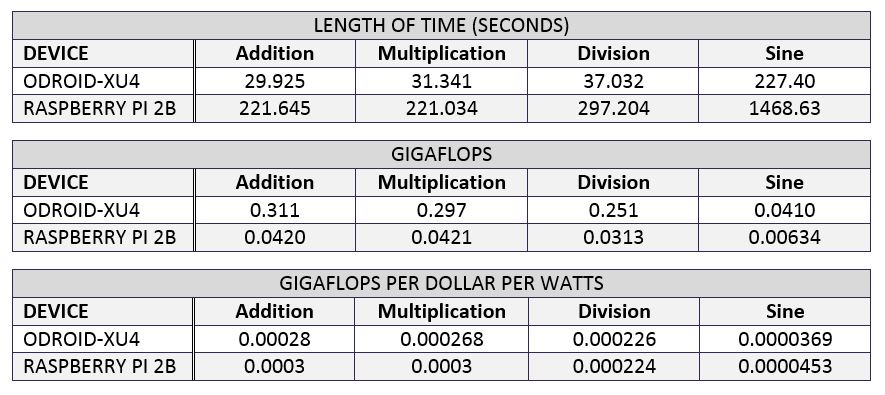
\includegraphics[width=0.75\textwidth]{pivsxu4table2.JPG}
\end{figure}

During the completion of this Sprint we encountered no significant failures. We were not set back from our schedule and were able to complete our Sprint goals.

\section{Sprint 2 Prototype}

This sprint also featured information gathering and preliminary work for knowlege we would need in creating the cluster. The decision was made to build the cluster out of ODroids, and the devices were ordered. The speed of the Ethernet port was tested while we waited for the devices to come in.

\subsection{Deliverable}

\begin{itemize}
\item Budget
\item Hardware Test
\item Switch Benchmark
\item Ethernet Benchmark
\item USB to Ethernet Benchmark
\item MPI Code
\item Message-Passing Protocol
\end{itemize}

\subsection{Backlog}

\begin{itemize}
\item Build the cluster
\item Code for the cluster
\item Benchmark the cluster
\item Experiment with different topologies
\item Create a new mode of communication
\end{itemize}

\subsection{Success/Fail} 

However, the ODroids were backordered, and took two weeks longer than expected to arrive. In the meantime, we were able to test the speed of the Ethernet port with the ODroid that we had, and we tested the speed of a USB to Ethernet device. We found that direct Ethernet connection using the built in ports was about 750 Mbps, and the USB to Ethernet devices gave 450 Mbps.

\section{Sprint 3 Prototype}

The Cluster of eight ODroid XU4s was assembled, completing our first physical prototype. The ODroids were attached to a piece of plexiglass, along with a power supply with a 5 volt power cord for each ODroid, and an 8 port switch. The end result is pictured in the following figure. \\

\begin{figure}[tbh]
	\caption{Cluster in Star Topology.}
	\centering
		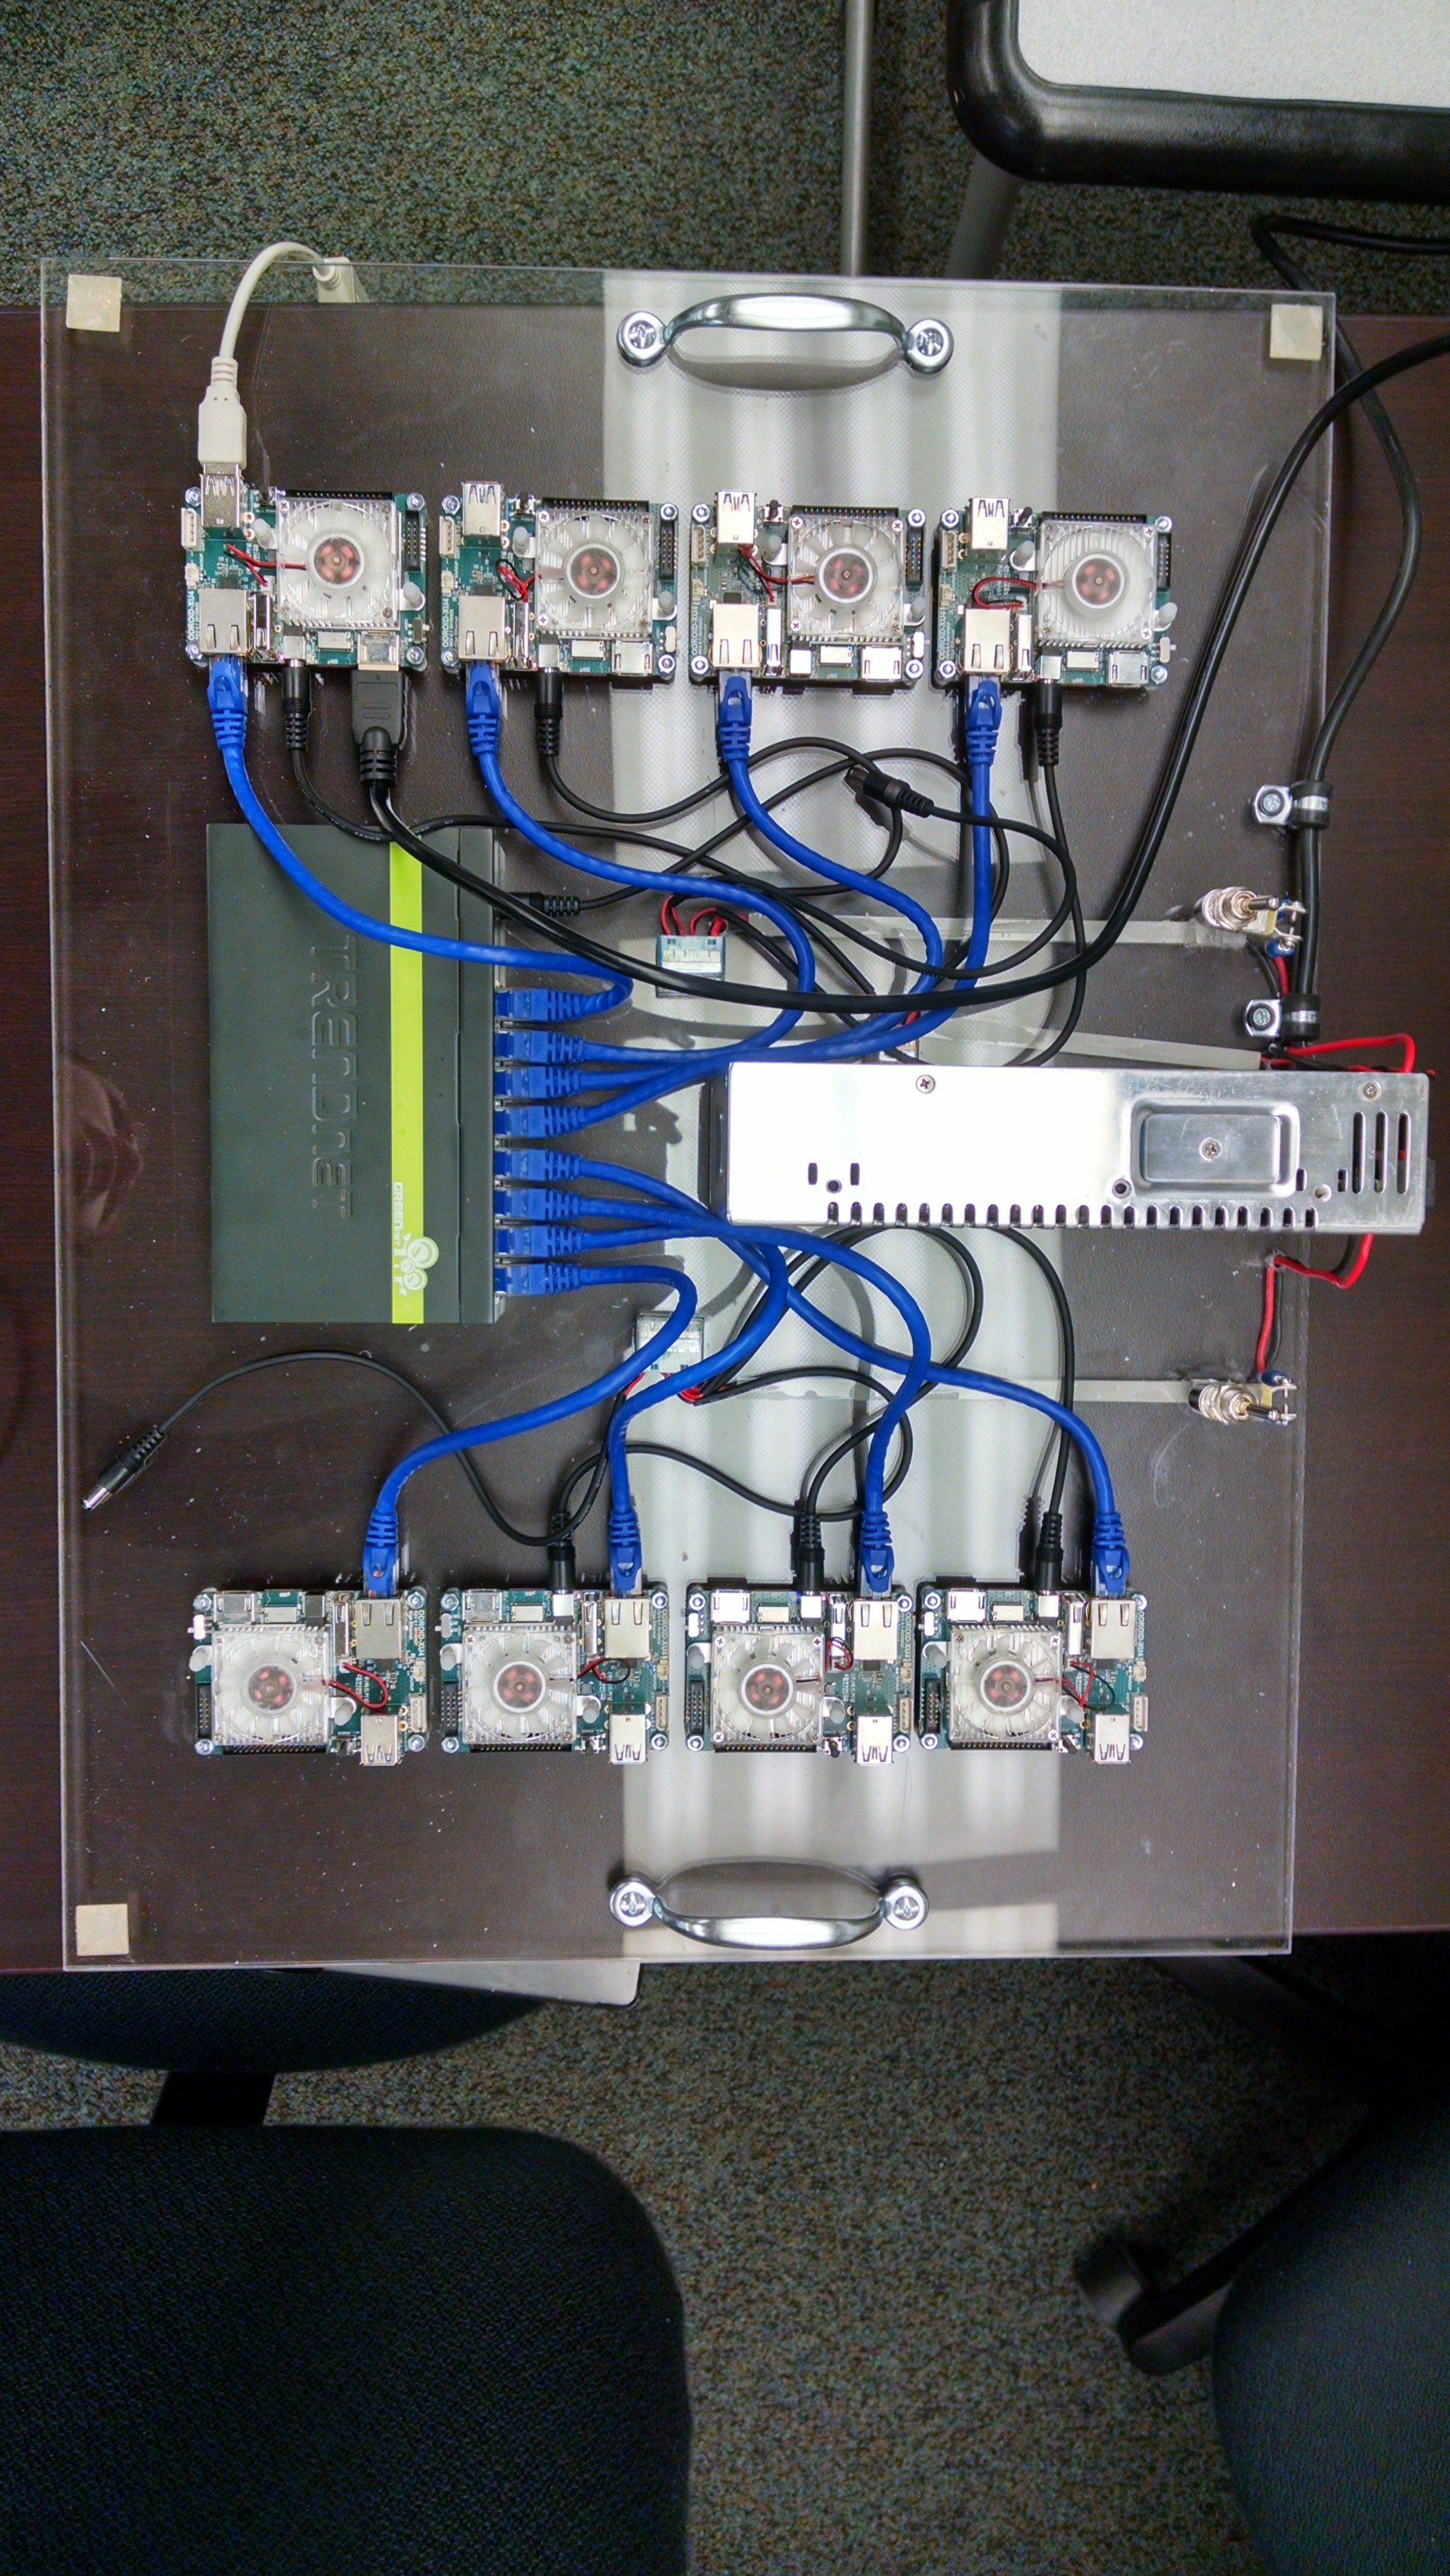
\includegraphics[width=0.75\textwidth]{IMG_20151201_104751350_HDR.jpg}
\end{figure}

On the software side, each ODroid was configured for our needs. First, each was assigned a static IP address in the network 192.168.0.X, and given it's hostname in accordinace with our naming convention of Snow White and the seven dwarfs. The final configuration for this sprint was to use RSA keys to allow each device to SSH to each other seven without prompting for a password. This was essential to allow MPI code to run. We also created some helper scripts to set up the cluster when it was booted. These included a script to use NFS to mount the /home directory of Snow White on the /home directory of the dwarfs. This was also essential to let MPI code located in the /home of Snow White to run on the cluster, as the same executable would be found in the same path on the dwarfs. We also created a script to shutdown the dwarfs from Snow White. 

\subsection{Deliverable}

\begin{itemize}
\item Built cluster
\item MPI code
\item Mounted home directory
\item Shutdown script
\item Mounting script
\item LINPACK and ATLAS installed on ODROIDs
\item MPI installed on ODROIDs
\item Hostnames
\item Fixed IP Addresses
\item SSH configuration
\end{itemize}

\subsection{Backlog}

\begin{itemize}
\item Research new connection methods
\item Benchmark the cluster
\item Experiment with different topologies
\item Create a new mode of communication
\item Design documentation
\item Research symposium
\begin{enumerate}
\item Complete abstract
\end{enumerate}
\item Design Fair
\end{itemize}

\subsection{Success/Fail}

We succeeded in creating and configured the cluster. Our largest failure was a setback from improperly changing the /etc/fstab file and causing the dwarfs to not boot. The goal was to make the devices mount the /home directory of Snow White on boot, but was ineffective. After a few days we were able to read the MMC card with a MMC to USB device and edit the fstab file manually using a different computer.

\section{Sprint 4 Prototype}

This sprint was largely the completion of benchmarking the cluster. We downloaned the source for High Performance Linpack, a tool used to test the speed of supercomputers. It worked with OpenMPI and ATLAS, a linear algebra package. We also had to build ATLAS for ARM. The benchmarking was a success and we found the speed of the cluster using all cores on all devices. Once that was complete, we began looking in to USB and GPIO communication.

\subsection{Deliverable}

\begin{itemize}
\item Graphs of total gigaflops performed depending on amount of devices used.
\item Debian package of LINPACK for ARM.
\item Found USB communication to not be feasible.
\item Able to send bits over GPIO between ODroid devices.
\item MICS abstract.
\end {itemize}

\subsection{Backlog}

\begin{itemize}
\item MICS presentation.
\item SDSMT Research Symnposium.
\item Design Documentation.
\item Design Fair.
\end{itemize}

\subsection{Success/Fail}

We successfully bencharked the cluster using Linpack. Results are shown in the following graph:

\begin{figure}[tbh]
	\caption{Linpack results.}
	\centering
		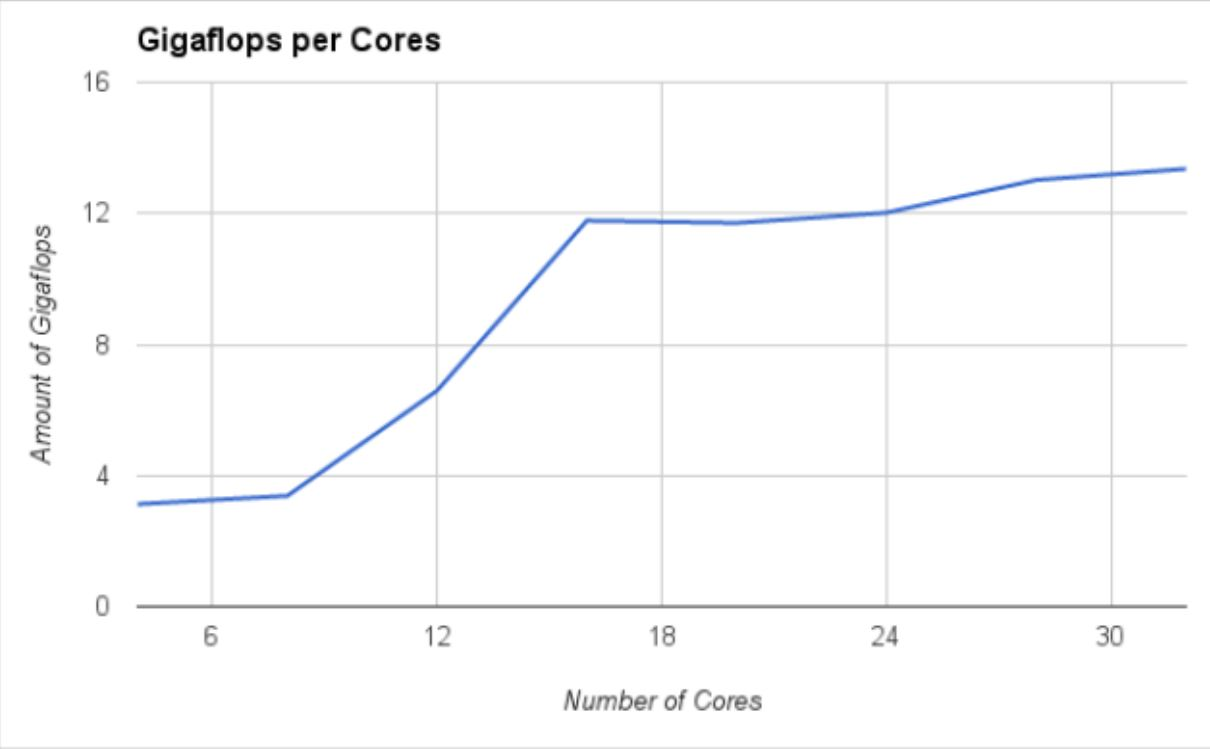
\includegraphics[width=0.75\textwidth]{minimalgraph.JPG}
\end{figure}

\section{Sprint 5 Prototype}

For this sprint, we tested the USB and GPIO communication. We were able to communicate over GPIO using the library WiringPi. In order to be able to do so, we had to install the source code on the ODROIDs and build it. We ran in to a few issues originally. First, the operatin system installed was not at it's most recent version, and therefore unable to work with the WiringPi libraries. We had to update each kernel individually, as shown in Figure~\ref{fig:purple} Once that was done, we still had to be able to use the library correctly. Extensive documentation existed for use with Raspberry Pis, but not for ODROID XU4s. Therefore, through a process of trial and error to see which WiringPi pin number corresponded to each physical pin, we were able to create our own in Figure~\ref{fig:gpio} \\

\begin{figure}[tbh]
	\caption{Linpack results.}
	\centering
		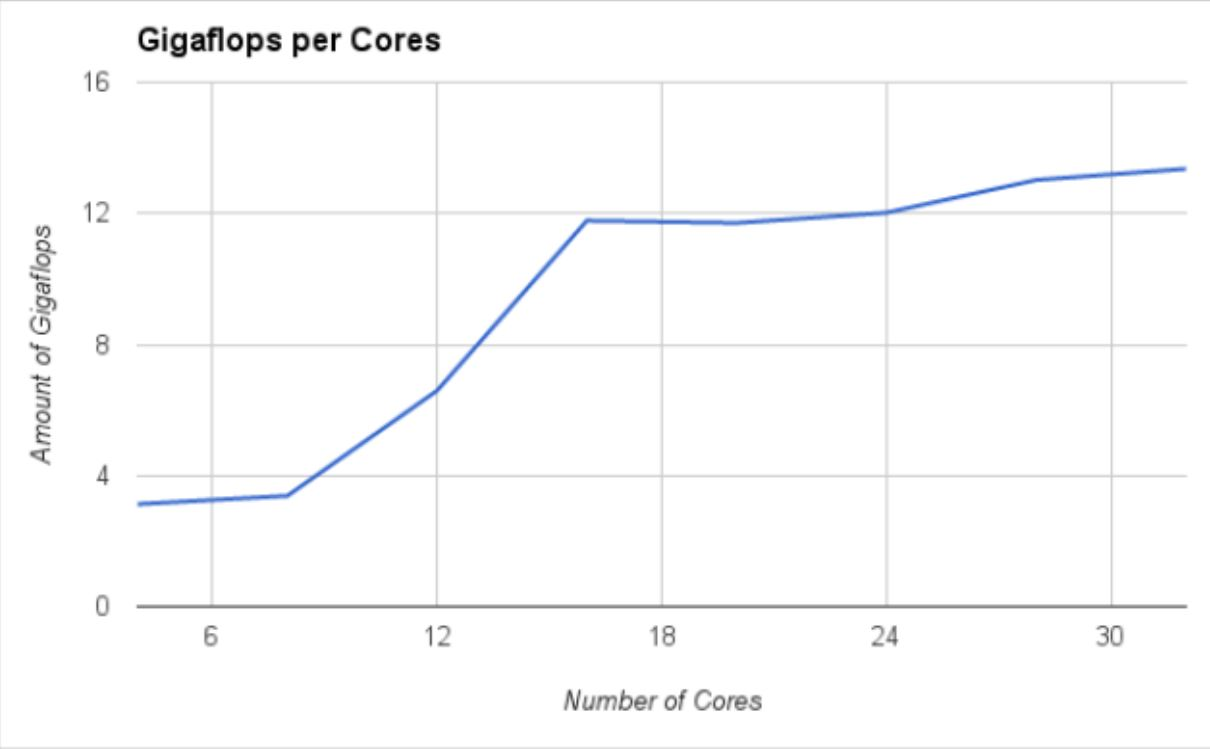
\includegraphics[width=0.75\textwidth]{minimalgraph.JPG}
	\label{fig:minimal}
\end{figure}

\begin{figure}[tbh]
	\caption{Updating kernel.}
	\centering
		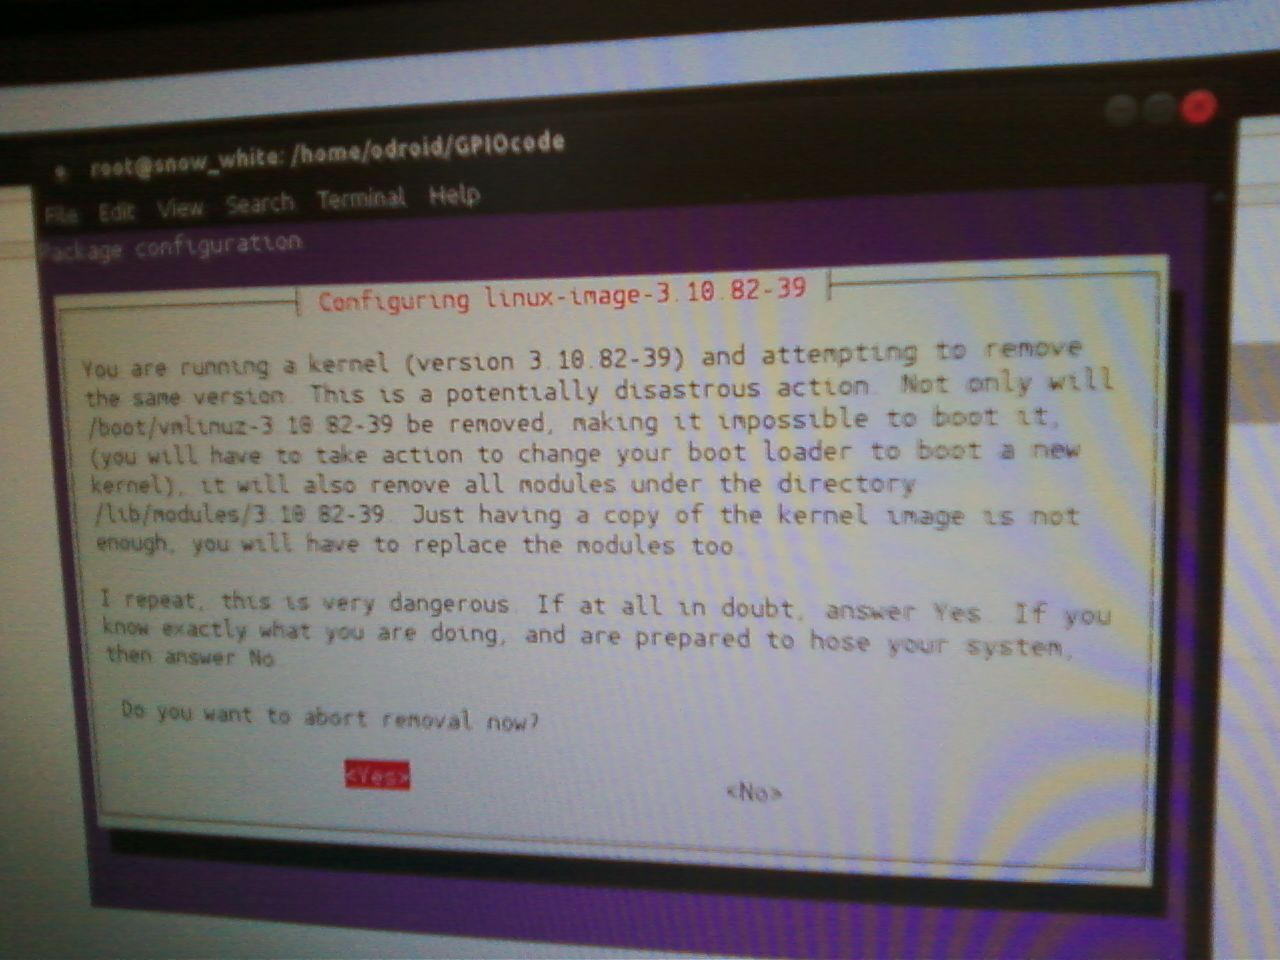
\includegraphics[width=0.75\textwidth]{PurpleScreen.jpg}
	\label{fig:purple}
\end{figure}

\begin{figure}[tbh]
	\caption{WiringPi values.}
	\centering
		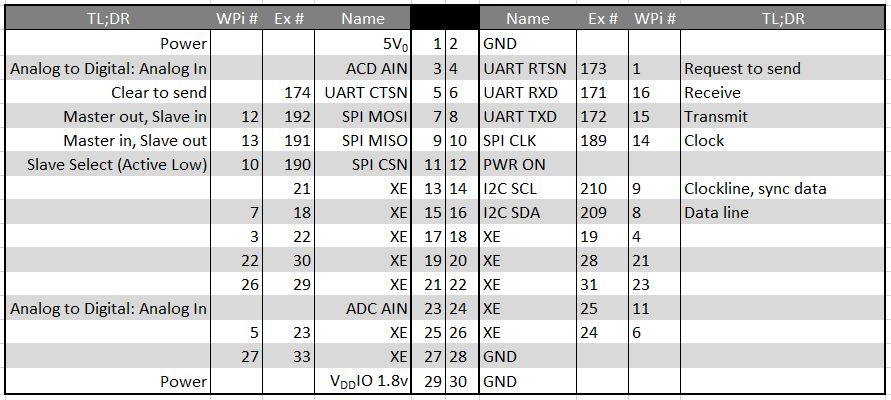
\includegraphics[width=0.75\textwidth]{gpio.JPG}
	\label{fig:gpio}
\end{figure}

It was determined that netiher were pratcical for our purposes due to the scope of the project and the low speed. In order to try and increase the gigaflops of the system, we instead experimented with different topologies. We used USB to Ethernet devices to add more network interfaces to each ODroid and attach them in a ring. This allowed a different method of communication instead of using the switch. In order for communication to work, we had to assign IP addresses to the new interfaces on the 192.168.X.Y network, where X is the ODroid number 0-7, and Y was the number of the interface for that device. We also created our abstract for the SDSMT Reseach Symposium, and for the MICS conference. We wrote a first draft of the MICS paper as well in preparation of our presentation in April 23rd. 

\subsection{Deliverable}

\begin{itemize}
\item Design for the hypercube and ring topology.
\item Routing tables for each of the ODROIDs.
\item The cluster connected with new topology.
\item Able to send bits over GPIO between ODroid devices.
\item Acceptance into MICS.
\item First draft of MICS paper.
\item SDSMT Research Symposium abstract.
\end{itemize}

\subsection{Backlog}

\begin{itemize}
\item MICS presentation.
\item SDSMT Research Symnposium.
\item Completed hypercube cluster.
\item Conglomerate data results.
\item Design Documentation.
\item Design Fair.
\end{itemize}

\subsection{Success/Fail}

Our largest failure this sprint was our inability to benchmark the different topologies. We found that MPI does not work with different network interfaces on the same subnet. Even after changing the IP addresses so that each IP address was on a different subnet, the code still did not work. Therefore, we are unable to use Linpack to benchmark the cluster in the ring or hypercube topology.
